\documentclass[12pt, notitlepage]{article}
\usepackage[utf8]{inputenc}
\usepackage{graphicx}
\graphicspath{ {images/} }

\usepackage[english]{babel}
\usepackage[nottoc]{tocbibind}

\usepackage{hyperref}
\usepackage[left=3cm,right=3cm,top=2cm,bottom=2cm]{geometry}

\usepackage{bbm}

\usepackage{amsmath}
\usepackage{amsthm}
\usepackage{amsfonts}
\usepackage{amssymb}
\newtheorem{thm}{Theorem}[section]
\newtheorem{lem}[thm]{Lemma}
\newtheorem{prop}[thm]{Proposition}
\newtheorem{cor}[thm]{Corollary}
\newtheorem{conj}[thm]{Conjecture}
\newtheorem{exmp}[thm]{Example}
\newtheorem{remark}[thm]{Remark}

\usepackage{mathtools}
\usepackage{tikz-cd}

\usepackage{xcolor}

\theoremstyle{definition}
\newtheorem{defn}{Definition}[section]

\title{Proofs of some technical results in Homotopy Theory}
\author{Sayantan Khan}
\date{July 2017}

\usepackage{gentium}

\usepackage{todonotes}

\newcommand{\cat}[1]{\mathrm{#1}}
\newcommand{\cohomtheorie}{{h}^{\ast}}
\newcommand{\calz}{\mathcal{Z}}
\newcommand{\redco}{\widetilde{h}}
\newcommand{\dv}{\mathrm{DV}}
\newcommand{\coker}{\mathrm{coker}}

\makeatletter
\newcommand{\colim@}[2]{%
  \vtop{\m@th\ialign{##\cr
    \hfil$#1\operator@font colim$\hfil\cr
    \noalign{\nointerlineskip\kern1.5\ex@}#2\cr
    \noalign{\nointerlineskip\kern-\ex@}\cr}}%
}
\newcommand{\colim}{%
  \mathop{\mathpalette\colim@{\rightarrowfill@\textstyle}}\nmlimits@
}
\makeatother

\begin{document}
\maketitle

\tableofcontents

% \todototoc \listoftodos

\newpage

\section{Homotopy Excision Theorem}
\label{sec:hom-exc-theor}

The homotopy excision theorem is a fairly important and useful result in homotopy theory, and one of
its corollaries is the fundamental result in stable homotopy theory.

\subsection{Statement and proof of the excision theorem}
\label{sec:stat-proof-excis}

We'll need a lemma (without proof) and a couple of definitions before we state the theorem.

\begin{lem}[Long exact sequence of relative homotopy groups]
  For a pair $(X,A)$, the homotopy groups fit into the following long exact sequence.
  \begin{align*}
    \cdots \xrightarrow{\partial} \pi_q(A) \xrightarrow{i_{\ast}} \pi_q(X) \xrightarrow{j_{\ast}}
    \pi_q(X,A) \xrightarrow{\partial} \pi_{q-1}(A) \xrightarrow{i_{\ast}}\cdots
  \end{align*}
  The maps $i_{\ast}$ and $j_{\ast}$ are induced by the inclusions.
\end{lem}

\begin{defn}[$n$-connectivity for maps]
  A map $f$ from the pair $(X,A)$ to $(Y,B)$ is said to be $n$-connected if the induced map on the
  fundamental group $f_{\ast}: \pi_q(X,A) \to \pi_q(Y,B)$ is an isomorphism for $q < n$ and a
  surjection for $q=n$.
\end{defn}

\begin{defn}[$n$-connectivity for pairs]
  A pair $(X,A)$ is said to be $n$-connected if $i_{\ast}: \pi_0(A) \to \pi_0(X)$ is surjective and
  $\pi_q(X,A) = 0$ for all $q \leq n$. This is equivalent to saying that the inclusion map from
  $(A, \ast) \to (X, \ast)$ is $n$-connected (this follows from the long exact sequence for relative
  homotopy groups).
\end{defn}
With the terms defined, we can now state the theorem.

\begin{thm}[Homotopy excision]
  Let $X_1$ and $X_2$ be open subspaces of the space $X$, such that $X = X_1 \cup X_2$, and
  $X_0 = X_1 \cap X_2$ is not empty. If the pair $(X_1, X_0)$ is $m$-connected, and $(X_2, X_0)$ is
  $n$-connected, then the inclusion map $i: (X_1, X_0) \to (X, X_2)$ is $(m+n)$-connected, for
  $m \geq 1$ and $n \geq 0$.
\end{thm}
The idea of the proof is borrowed from May \cite{may} \todo[size=\tiny]{Put citation}: we will try to fit in
the maps we want to show are isomorphisms, and surjections into a long exact sequence, and try to
show that the third term vanishes in an appropriate range of dimensions. For this, we'll need
another form of homotopy groups.

\begin{defn}[Triad homotopy groups]
  If $X$ is a space, and $X_1$ and $X_2$ are open subspaces, such that the basepoint $x_0$ lies in
  $X_0 = X_1 \cap X_2$, then the triad homotopy groups are homotopy classes of maps of tetrads of
  the following form.
  \[
    \begin{tikzcd}
      &\left( I^q, I^{q-2} \times \{1\} \times I, I^{q-1} \times \{1\}, J^{q-2} \times I \cup I^{q-1} \times \{0\} \right) \ar[d] \\
      &(X, X_1, X_2, x_0) \\
    \end{tikzcd}
  \]
  This is only defined for $q \geq 2$.
\end{defn}

\begin{lem}[Long exact sequence of triad homotopy groups]
  The triad homotopy groups fit into a long exact sequence with relative homotopy groups in the
  following manner.
  \begin{align*}
    \cdots \xrightarrow{\partial} \pi_q(X_1, X_0) \xrightarrow{i_{\ast}} \pi_q(X, X_2)
    \xrightarrow{j_{\ast}} \pi_q(X; X_1, X_2) \xrightarrow{\partial} \pi_{q-1}(X_1, X_0) \xrightarrow{i_{\ast}} \cdots
  \end{align*}
  The maps $i_{\ast}$ and $j_{\ast}$ are induced by the inclusions, and $\partial$ is the boundary
  homomorphism, defined by restricting the map to the face of the cube corresponding to $X_1$.
\end{lem}
The proof that this sequence is exact is similar to the exactness proof for long exact sequence of
relative homotopy groups, and hence skipped.

Coming back to the excision theorem, we see that the condition $m \geq 0$ and $n \geq 0$ forces the
map at the level of $\pi_0$ to be an isomorphism. Furthermore, because $m \geq 1$, by an argument
similar to the one in the proof of Seifert--Van Kampen theorem, we get that $\pi_1(X, X_2) = 0$,
hence it's an isomorphism.  That means we only need to check for $2 \leq q \leq m+n$. By the long
exact sequence of triad homotopy groups, it's equivalent to proving the following theorem.
\begin{thm}
  With the same hypotheses as that of the homotopy excision theorem,
  \begin{align*}
    \pi_q(X; X_1, X_2) = 0
  \end{align*}
  for all $2 \leq q \leq m+n$.
\end{thm}

  \begin{proof}
    It will suffice to prove this result when $X$ is a CW complex, and $X_1$, $X_2$, and $X_0$ are
    CW subcomplexes.  That's because we can approximate a space by a CW complex up to homotopy, and
    that won't change the homotopy groups.  By our hypotheses on the connectivity of $(X_1, X_0)$
    and $(X_2, X_0)$, $(X_1, X_0)$ contains no relative $q$-cells i.e. $q$-cells outside $X_0$ for
    $q \leq m$, otherwise $\pi_q(X_1, X_0)$ wouldn't be $0$. Similarly, $(X_2, X_0)$ contains no
    relative $q$-cells for $q \leq n$. Furthermore, since we're trying to show a certain map from a
    compact space is nullhomotopic, it suffices to consider cases where $X$ is a finite CW complex.

    We will prove the result by inducting on the number of relative cells of $(X_1, X_0)$ and
    $(X_2, X_0)$. Since the base case is the hard part, we'll show the induction step first. Suppose
    we know the result for the triads $(X; X_1', X_2)$ and $(X; X_1, X')$, where $X_1$ is obtained
    by attaching one more cell to $X_1'$, and $X' = X_1' \cup_{X_0} X_2$ (The first triad satisfies
    the induction hypothesis for obvious reasons. The second triad has one relative cell in each
    component, so that reduces to the base case.).
     
    By the long exact sequence of a triple, we get exactness in the rows of the following diagram.
    \[
      \begin{tikzcd}
        \pi_q(X_1', X_0) \ar[d, "\alpha"] \ar[r] & \pi_q(X_1, X_0) \ar[d, "\beta"], \ar[r] &
        \pi_q(X_1, X_1') \ar[d, "\gamma"] \ar[r] & \pi_{q-1}(X_1', X_0) \ar[d, "\delta"] \\
        \pi_q(X', X_2) \ar[r] & \pi_q(X, X_2) \ar[r] & \pi_q(X, X') \ar[r] & \pi_{q-1}(X', X_2) \\
      \end{tikzcd}
    \]
    By the induction hypothesis, the maps $\alpha$ and $\gamma$ are surjective, and $\delta$ is
    injective, which means the map $\beta$ is surjective. This shows that $\pi_q(X; X_1, X_2) = 0$.

    Similarly, if we know the result for $(X; X_1, X_2')$ and $(X; X', X_2)$, where $X_2$ is
    obtained by attaching one more cell to $X_2'$, then we have the result for $(X; X_1, X_2)$,
    since the map $i: (X_1, X_0) \hookrightarrow (X, X_2)$ factors through in the following manner.
    \begin{align*}
      (X_1, X_0) \xhookrightarrow{i_1} (X', X_2') \xhookrightarrow{i_2} (X, X_2)
    \end{align*}
    By the induction hypothesis, both ${i_1}_{\ast}$ and ${i_2}_{\ast}$ are surjections, hence their
    composite $i_{\ast}$ is a surjection.

    All that is left now is to prove the base case, i.e. when both $(X_1, X_0)$ and $(X_2, X_0)$
    have one relative cell. Without loss of generality, let $X_1 = X_0 \cup D^k$, where $k > m$ and
    $X_2 = X_0 \cup D^l$, where $l > n$. We need to show that the associated map of tetrads is
    nullhomotopic.
    \[
      \begin{tikzcd}
        &\left( I^q, I^{q-2} \times \{1\} \times I, I^{q-1} \times \{1\}, J^{q-2} \times I \cup I^{q-1} \times \{0\} \right) \ar[d] \\
        &(X, X_0 \cup D^k, X_0 \cup D^l, x_0) \\
      \end{tikzcd}
    \]

    Pick interior points $x_1 \in D^k$ and $x_2 \in D^l$. We then have the following maps of triads.
    \begin{align}
      (X_1; X_1, X_1 - x_1) &\hookrightarrow (X - x_2; X_1, X - \{x_1, x_2\}) \label{eq:1} \\
      (X - x_2; X_1, X - \{x_1, x_2\}) &\hookrightarrow (X; X_1, X - \{x_1\}) \label{eq:2} \\
      (X; X_1, X_2) &\hookrightarrow (X; X_1, X - \{x_1\}) \label{eq:3}
    \end{align}
    The maps labelled \ref{eq:1} and \ref{eq:3} induce isomorphisms at the level of triad homotopy
    groups.  This is easy to see after observing the fact that $D^n$ with an interior point removed
    can be homotoped to its boundary $S^{n-1}$. Doing this to the associated disks in map \ref{eq:1}
    and \ref{eq:3}, we see the isomorphisms. Furthermore, $\pi_q(X_1; X_1, X_1 - x_1) = 0$ for
    $q \geq 2$: this follows trivially from the long exact sequence of triad homotopy groups. That
    means if we show map \ref{eq:2} induces a surjection at the level of $\pi_{\ast}$, we'll be
    done.

    Pick any map of tetrads $f$ going into $(X; X_1, X - \{x_1\})$. We need to show $f$ is homotopic
    to a map into $(X - x_2; X_1, X - \{x_1, x_2\})$ followed by the inclusion map \ref{eq:2}. Let
    $D^k_{1/2}$ and $D^l_{1/2}$ be sub-disks of radius $\frac{1}{2}$. Using the compactness of
    $I^q$, it's easy to divide $I^q$ into smaller sub-cubes $I^q_{\alpha}$ such that if
    $f(I^q_{\alpha})$ intersects $D^k_{1/2}$, it's contained in the interior of $D^k$ and if it
    intersects $D^l_{1/2}$, it's contained in the interior of $D^l$. By simplicial approximation, we
    can make $f$ homotopic (as a map of tetrads) to a map $g$ whose restriction to the $(k-1)$
    skeleton of $I^q$ (with its subdivided cubes as cells) (the $(k-1)$ skeleton could possibly be
    empty as well) does not cover $D^k_{1/2}$, and similarly, whose restriction to $(l-1)$-skeleton
    does not cover $D^l_{1/2}$. Furthermore, we can make sure that we pick an $x_2$ in $D^l_{1/2}$
    such that $g^{-1}(x_2)$ has dimension at most $q-l$ and it does not lie in the image of the
    $(l-1)$-skeleton. Although, this is intuitively clear, it requires some work, but that will just
    obscure the proof, so we leave it be.

    Let $\pi: I^q \to I^{q-1}$ be a projection map that discards the last coordinate, and let $K$ be
    the following space.
    \begin{align*}
      K = \pi^{-1} \circ \pi \circ g^{-1} (x_2)
    \end{align*}
    This means $K$ has dimensions at most $1$ more than $g^{-1}(x_2)$. We have the following
    inequalities.
    \begin{align*}
      \dim K &\leq \dim g^{-1}(x_2) + 1 \\
             &\leq q - l + 1 \\
             &< m + 1
    \end{align*}
    The last inequality follows since $l > n$, and $q \leq m+n$. And since $m < k$, and all our
    dimensions are integers, that lets us directly conclude $\dim K \leq k - 1$. This means $g(K)$
    does not cover all of $D^k_{1/2}$. We pick $x_1 \in D^k_{1/2}$ such that it does not lie in
    $g(K)$. It's not too hard to see that $\pi(g^{-1}(x_1)) \cup \partial I^{q-1}$ and
    $\pi(g^{-1}(x_2))$ are disjoint (drawing a picture in the case of $I^3$ helps visualizing the
    scenario)\todo[size=\tiny]{Insert image perhaps?}. Both of these are closed subsets of
    $I^{q-1}$, hence by Uryssohn's lemma, there exists a function $v: I^{q-1} \to I$ such that the
    following equalities are satisfied.
    \begin{align*}
      v(\pi(g^{-1}(x_1)) \cup \partial I^{q-1}) &= 0 \\
      v(\pi(g^{-1}(x_2))) &= 1
    \end{align*}
    We use this to define a map $h$ from $I^{q+1}$ to $I^q$.
    \begin{align*}
      h(r, s, t) = (r, s - s \cdot t \cdot v(r))
    \end{align*}
    Let $f': I^q \to X$ be defined as $f'(r,s) = g \circ h(r,s, 1)$.  We have the following
    observations.
    \begin{align*}
      h(r,s,0) &= (r,s) \\
      h(r,0,t) &= (r, 0) \\
      h(r,s,t) &= (r,s) &&\text{if $r \in \partial I^{q-1}$}
    \end{align*}
    Furthermore, if $h(r,s,t) \in g^{-1}(x_1)$, then $v(r) = 0$, and hence $h(r,s,t) = (r,s)$.
    Similarly, $h(r,s,t) \in g^{-1}(x_2)$ implies $v(r)= 1$, and $h(r,s,t) = (r, s-st)$. Thus,
    $g \circ h$ is the required homotopy of tetrads.
    
  \end{proof}
  
  \subsection{Corollaries of the excision theorem}
  \label{sec:coroll-excis-theor}

  \subsubsection{Freudenthal suspension theorem}
  \label{sec:freud-susp-theor}

  For any space $X$, we have the suspension homomorphism, $\Sigma_{\ast}$, defined as follows.
  \begin{align*}
    \Sigma_{q}: \pi_q(X) &\to \pi_{q+1}(\Sigma X) \\
    \Sigma_{q}([f]: S^q \to X) &= [f \wedge \mathrm{id}]
  \end{align*}
  Under certain additional conditions on the space $X$ and $q$, $\Sigma_q$ is an isomorphism.  The
  excision theorem lets us easily deduce what those conditions are.

\begin{thm}[Freudenthal suspension]
  If $X$ is $n$-connected, then the suspension homomorphism is an isomorphism for $q \leq 2n$ and a
  surjection for $q = 2n+1$.
\end{thm}

\begin{proof}
  Let $C_+X$ and $C_-X$ be the upper and lower cones of $\Sigma X$. Their intersection is $X$.  The
  pairs $(C_+X, X)$ and $(C_-X, X)$ are both $n$-connected (this follows from the fact that cones
  are contractible, and the long exact sequence of relative homotopy groups). By the homotopy
  excision theorem, we get that the inclusion of $(C_+X, X)$ into $(\Sigma X, C_-X)$ is an
  isomorphism until $\pi_{2n}$ and a surjection for $\pi_{2n+1}$. Again, using the long exact
  sequence of relative homotopy groups, we get that $\pi_{\ast}(C_+X, X) \cong \pi_{\ast}(X)$, and
  similarly $\pi_{\ast}(\Sigma X, C_-X) \cong \pi_{\ast+1}(\Sigma X)$. There is a bit of work
  involved in showing that this isomorphism/surjection is actually the suspension homomorphism, but
  that's technical, and not too hard.
\end{proof}

\subsubsection{Stable homotopy}
\label{sec:stable-homotopy}

We now look at the colimit of the following diagram.
\begin{align*}
  \pi_q(S^0) \xrightarrow{\Sigma_q} \pi_{q+1}(S^1) \xrightarrow{\Sigma_{q+1}} \pi_{q+2}(S^2) \xrightarrow{\Sigma_{q+2}} \cdots
\end{align*}
Since $S^n$ is $n$-connected, after $\frac{q}{2}$ steps, the arrows in the diagram become
isomorphisms, which means the colimit of the diagram is what the diagram stabilizes to after
$\frac{q}{2}$ steps. We call the colimit the $q$\textsuperscript{th} stable homotopy group of
$S^0$. From this point on, it's not too hard to show that the stable homotopy functor is a nicely
behaved functor: in fact, it's a generalized homology theory.
  
\section{Comparison theorem for cohomology theories}
\label{sec:comp-theor-cohom}

\begin{thm}[Comparison Theorem]
  If $h$ and $k$ are two reduced cohomology theories satisfying the $(\mathrm{DV})$ axiom, such that
  there exists a natural transformation $\chi$ from $h^{\ast}$ to $k^{\ast}$ and $\chi$ induces a
  natural isomorphism from $h^n(S^0)$ to $k^n(S^0)$ for all $n$, then $\chi$ is a natural
  isomorphism of cohomology theories.
\end{thm}

\begin{proof}
  First, we'll use a simple reduction. For any pointed space $X$, we'll show if $\chi$ is an
  isomorphism from $h^n(X_+)$ to $k^n(X_+)$, then $\chi$ is an isomorphism between $h^n(X)$ and
  $k^n(X)$.  Here, $X_+$ is the space $X \amalg {+}$, with the basepoint being $+$. Consider the
  following cofiber sequence.
  \begin{align*}
    S^0 \xrightarrow{i} X_+ \xrightarrow{} X
  \end{align*}
  The map from $S^0$ to $X_+$ sends the basepoint of $S^0$ to $+$, and the other point to the
  original basepoint of $X$. This cofiber sequence splits, which means an isomorphism from
  $h^n(X_+)$ to $k^n(X_+)$ is equivalent to an isomorphism from $h(X)$ to $k(X)$ (by the five
  lemma).

  The next step in the proof is to show the isomorphism for finite CW complexes. This will be done
  by showing the isomorphism for $S^n$ and $D^n$ for all $n$, and then using the fact that all
  finite CW complexes are pushouts of disks and spheres. We have an isomorphism on all spheres from
  the suspension isomorphism, and that extends to wedges of spheres. And since all disks are
  contractible, we have an isomorphism there as well. This also tells us that $\chi$ is an
  isomorphism from $0$-dimensional CW complexes. We'll proceed by induction at this point. An $n$
  skeleton is defined by the following pushout.
  \[
    \begin{tikzcd}
      \coprod S_+^n \ar[d] \ar[r] & X^{(n-1)}_+ \ar[dashrightarrow, d] \\
      \coprod D_+^n \ar[dashrightarrow, r] & X^{(n)}_+ \\
    \end{tikzcd}
  \]
  We then apply the Mayer-Vietoris sequence to the subspaces $\coprod D_+^n$ and $X^{(n-1)}_+$. Call
  these subspaces $T_1$ and $T_2$. Their intersection $T_0$ is the wedge of spheres.
  \[
    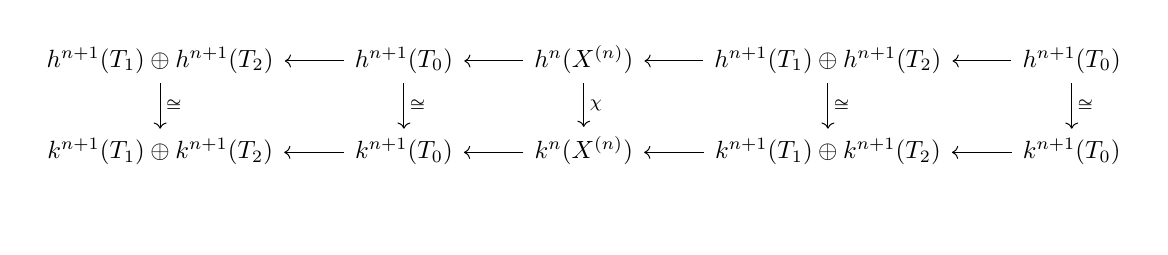
\begin{tikzpicture}[baseline= (a).base]
      \node[scale=.90] (a) at (0,0){
        \begin{tikzcd}
          h^{n+1}(T_1) \oplus h^{n+1}(T_2) \ar[d , "\cong"] & h^{n+1}(T_0) \ar[l] \ar[d , "\cong"]& h^n(X^{(n)}) \ar[l] \ar[d, "\chi"] & h^{n+1}(T_1) \oplus h^{n+1}(T_2) \ar[l] \ar[d , "\cong"]& h^{n+1}(T_0) \ar[l] \ar[d , "\cong"]\\
          k^{n+1}(T_1) \oplus k^{n+1}(T_2) & k^{n+1}(T_0) \ar[l] & k^n(X^{(n)}) \ar[l] & k^{n+1}(T_1) \oplus k^{n+1}(T_2) \ar[l] & k^{n+1}(T_0) \ar[l] \\
        \end{tikzcd}
      };
    \end{tikzpicture}
  \]
  By the induction hypothesis, all but the middle arrows are isomorphisms, hence by the five lemma,
  $\chi$ is an isomorphism too. This shows $\chi$ is a natural isomorphism for finite dimensional CW
  complexes.

  The final step is to show this for infinite dimensional CW complexes. This will require the use of
  Milnor's theorem \ref{thm-milnor}. For any infinite dimensional CW complex $X$, take the
  filtration consisting of its finite dimensional skeletons. Then we have maps between the following
  short exact sequences.
  \[
    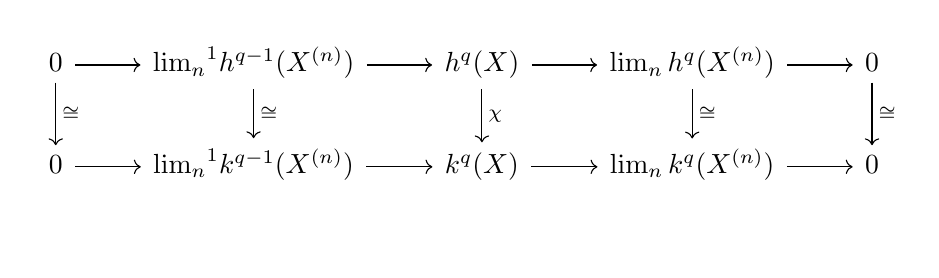
\begin{tikzpicture}
      \node[scale=1] (a) at (0,0) {
        \begin{tikzcd}
          0 \ar[r] \ar[d, "\cong"] & {\lim_n}^1 h^{q-1}(X^{(n)}) \ar[r] \ar[d, "\cong"]& h^q(X) \ar[r] \ar[d, "\chi"] & \lim_n h^q(X^{(n)}) \ar[r] \ar[d, "\cong"]& 0 \ar[d, "\cong"]\\
          0 \ar[r] & {\lim_n}^1 k^{q-1}(X^{(n)}) \ar[r] & k^q(X) \ar[r] & \lim_n k^q(X^{(n)}) \ar[r] & 0 \\
        \end{tikzcd}
      };
    \end{tikzpicture}
  \]
  By the proof for the finite dimensional case, we have the all but the middle arrow are
  isomorphisms. By the five lemma, we get the middle arrow is an isomorphism too, which concludes
  the proof.
  
\end{proof}

\section{Brown's representability theorem}
\label{sec:browns-repr-theor}

In this section, we shall see that all reduced cohomology theories that satisfy the wedge sum
($\dv$) axiom are representable functors, i.e. they are naturally isomorphic to the hom functor in
the homotopy category $\cat{hCW}_{\ast}$. In particular, for a given reduced cohomology theory
$\cohomtheorie$, we'll construct a sequence of spaces $\calz(n)$, which we'll call a spectrum, such
that $\redco^n(X)$ is naturally isomorphic to $\left[X, \calz(n)\right]$.

\subsection{Spectra and cohomology theories}
\label{sec:spectra-cohom-theor}

\begin{defn}[$\Omega$-Spectrum]
  A spectrum is a $\mathbb{Z}$ indexed sequence of pointed spaces $\calz(n)$ together with structure
  maps $\sigma_n: \Sigma \calz(n) \to \calz(n+1)$. If the adjoints of the structure maps, i.e. the
  maps $\widetilde{\sigma}_n: \calz(n) \to \Omega \calz(n+1)$ are homotopy equivalences, then the
  spectrum is called an $\Omega$-spectrum.
\end{defn}

\begin{prop}
  Given a $\Omega$-spectrum $\calz$, one can define the following functor.
  \begin{align*}
    \redco^n(X; \calz) = \left[X, \calz(n)\right]
  \end{align*}
  This is a contravariant functor which satisfies the homotopy invariance $(\mathrm{H})$, suspension
  $(\mathrm{S})$, exactness $(\mathrm{E})$, and the wedge sum $(\dv)$ axiom. It is therefore a
  reduced cohomology theory.
\end{prop}

\begin{proof}
  We'll deal with the axioms one at a time.
  \begin{description}
  \item[Homotopy invariance (H):] This is obvious, because we are looking at homotopy classes of
    maps.
  \item[Suspension (S):] We need to show there is a natural isomorphism from $\redco^n(X)$ to
    $\redco^{n+1}(\Sigma X)$. Note that the adjoint of the structure maps are homotopy equivalences.
    We therefore have a natural isomorphism.
    \begin{align*}
      \left[ X, \calz(n) \right] \cong \left[ X, \Omega \calz(n+1) \right]
    \end{align*}
    On the other hand, since $\Sigma$ are $\Omega$ are adjoints, we have the following natural
    isomorphism.
    \begin{align*}
      \left[ X, \Omega \calz(n+1) \right] \cong \left[ \Sigma X, \calz(n+1) \right]
    \end{align*}
    Composing the two natural isomorphisms, we get our required isomorphism.
  \item[Exactness (E):] We need to show for any cofibration $i: A \hookrightarrow X$, the following
    sequence is exact.
    \begin{align*}
      \redco^n(A) \leftarrow \redco^n(X) \leftarrow \redco^n\left( X/A \right)
    \end{align*}
    Using the cofiber sequence, we get that following sequence is exact.
    \begin{align*}
      [A, \calz(n)] \leftarrow [X, \calz(n)] \leftarrow \left[\left(X/A\right), \calz(n) \right]
    \end{align*}
  \item[Wedge sum (DV):] The functor $[\cdot, \calz(n)]$ satisfies $(\dv)$ axiom. This is fairly
    easy to check. That means $\redco^{\ast}$ satisfies $(\dv)$ axiom.
  \end{description}
\end{proof}

\todo[size=\tiny]{To construct easy examples of spectra, one needs to check that the filtered
  colimits commute with the loop space functor, at least for nice enough spaces.}
% {\color{red} To construct easy examples of spectra, one needs to check that filtered colimits
% commute with the loop space functor, at least for nice enough spaces.}

\subsection{Proof of Brown's representability theorem}
\label{sec:proof-browns-repr}

\textbf{Note:} This proof is primarily taken from A. J. Tolland's article\cite{tolland}.

In the previous section, we saw that if we are given an $\Omega$-spectrum, we can construct a
reduced cohomology theory using the spectrum. Brown's representability theorem is the converse of
the previous theorem, i.e. given a reduced cohomology theory which satisfies the $(\dv)$ axiom, it
can be represented by an $\Omega$-spectrum, which is unique up to homotopy. This theorem is fairly
technical, and will require the use of the theorem on Milnor exact sequence (theorem
\ref{thm-milnor}).

\begin{thm}[Brown's representability theorem]
  Let $\redco^{\ast}$ be a reduced cohomology theory satisfying the $(\dv)$ axiom. Then there is an
  $\Omega$-spectrum $\calz$ such that $\redco^{n}$ is naturally isomorphic to
  $\left[\cdot, \calz(n) \right]$.
\end{thm}

\begin{proof}
  The proof will have two main parts. The first part will involve constructing the spaces $\calz(n)$
  for each $n$ such that there is a natural isomorphism from $\redco^n(X)$ to
  $\left[ X, \calz(n) \right]$ for all CW complexes $X$. The second part will involve constructing
  the structure maps from $\Sigma \calz(n) \to \calz(n+1)$.

  Fix an $n \in \mathbb{Z}$. We will construct the space $\calz(n)$ as a CW complex, using finite
  dimensional skeletons $\calz(n)_k$. For each $k$, we will also pick a cohomology class $c_n(k)$ in
  $\redco^n(\calz(n)_k)$ such that the map
  $d_n^{m}(k): \left[S^m, \calz(n)_k \right] \to \redco^n(S^m)$ is an isomorphism for $m < k$ and
  surjection for $m=k$ \todo[size=\tiny]{Show that this is a group homomorphism for $m \geq 1$}.
  \begin{align*}
    d_n^{m}(k) &: \left[ S^m, \calz(n)_k\right] \to \redco^n(S^m) \\
    d_n^{m}(k) &: [f] \mapsto f^{\ast}(c_n(k))
  \end{align*}
  For $k=0$, we define $\calz(n)_0$ as follows.
  \begin{align*}
    \calz(n)_0 := \bigvee_{\alpha \in \redco^n(S^0)} S_{\alpha}^0
  \end{align*}
  The cohomology group of $\calz(n)_0$ is given by a direct product, since $\redco^n$ satisfies the
  $\mathrm{(DV)}$ axiom.
  \begin{align*}
    \redco^n(Z(n)_0) \cong \prod_{\alpha \in \redco^n(S^0)} \redco^n(S_{\alpha}^0)
  \end{align*}
  Pick the following element as $c_n(0)$.
  \begin{align*}
    c_n(0) := \prod_{\alpha \in \redco^n(S^0)} \alpha
  \end{align*}
  Since $k=0$, we only need to show that $d_n^0(0)$ is a surjection. Pick any
  $\alpha \in \redco^n(S^0)$.  Corresponding to this $\alpha$, there's a copy of $S^0$ sitting
  inside $\calz(n)_0$. Let $f$ be the inclusion map of this copy of $S^0$ into $\calz(n)_0$. Then
  the induced map on cohomology is the projection map on the $\alpha$\textsuperscript{th}
  coordinate, since the cohomology theory satisfies the $(\dv)$ axiom. Applying this induced map on
  $c_n(0)$, we see that in the $\alpha$\textsuperscript{th} coordinate, it has $\alpha$, because of
  the way we defined it.  This shows the map is surjective.

  To prove the induction step, suppose we have defined the space $\calz(n)_k$ and $c_n(k)$ that
  satisfy the required properties. Let $K_k \trianglelefteq \left[ S^k, \calz(n)_k \right]$
  \todo[size=\tiny]{The cofibration probably works if you take a subset of $K_k$ that does not
    contain the constant map} be the kernel of the map $d_n^k(k)$.  We construct the following map.
  \begin{align*}
    \phi_n(k): \bigvee_{x \in K_k} S^k \to \calz(n)_k \vee \bigvee_{y \in \redco^n(S^{k+1})} S^{k+1}
  \end{align*}
  This map is obtained by taking the wedge of maps from $S^k$ to $\calz(n)_k$ which are contained in
  $K_k$.  This is a cofibration \todo[size=\tiny]{Not sure how to show this, or whether this is
    entirely correct. Need to check later}. By the $(\dv)$ axiom, we have the following cohomology
  groups.
  \begin{align*}
    \redco^n \left( \calz(n)_k \vee \bigvee_{y \in \redco^n(S^{k+1})} S^{k+1} \right) = \redco^n(\calz(n)_k) \times \prod_{y \in \redco^n(S^{k+1})} \redco^n(S^{k+1})
  \end{align*}
  From this, we can immediately see that the elements of
  $\redco^n \left( \calz(n)_k \vee \bigvee_{y \in \redco^n(S^{k+1})} S^{k+1} \right)$ of the form
  $(c_n(k), \bullet)$ (where $\bullet$ is any arbitrary element) is in the kernel of
  $\phi_n^{\ast}(k)$.  Define $\calz(n)_{k+1}$ to be the cofiber of the map $\phi_n(k)$, and let the
  map to the cofiber be $b_n(k)$.  By the exactness axiom, we have that the following sequence is
  exact.
  \begin{align*}
    \redco^n(\calz(n)_{k+1}) \xrightarrow{b_n^{\ast}(k)}  \redco^n(\calz(n)_k) \times \prod_{y \in \redco^n(S^{k+1})} \redco^n(S^{k+1})
    \xrightarrow{\phi_n^{\ast}(k)} \prod_{x \in K_k} \redco^n(S^k)
  \end{align*}
  Pick the following element $A \in \prod_{y \in \redco^n(S^{k+1})} \redco^n(S^{k+1})$.
  \begin{align*}
    A := \prod_{\alpha \in \redco^n(S^{k+1})} \alpha
  \end{align*}
  The element $(c_n(k), A)$ lies in the kernel of $\phi_n^{\ast}(k)$, which means it lies in the
  image of $b_n^{\ast}(k)$. We define $c_n(k+1)$ to be a pre-image of $(c_n(k), A)$. Seeing that the
  associated map $d_n^m(k+1)$ is surjective for $m=k+1$ is easy enough. The proof is the same as
  that in the case of $d_n^0(0)$.\todo[size=\tiny]{Maybe write the proof anyways. See if it adds to
    the clarity at all} The trickier part is showing injectivity for $m < k+1$. Since $d_m^n(k)$ is
  a group homomorphism (for $M \geq 1$), for $m \geq 1$, it will suffice to show the kernel is
  trivial.  \todo[size=\tiny]{I'm skipping the proof of the case when $m=0$. I think it should be
    fairly easy once I figure out why the map is a cofibration.}  Pick an element, say $[f]$ in the
  kernel. We need to show that $f$ is a nullhomotopic map. But at each step, we coned off the kernel
  of $d_n^m(m)$. That means $f$ is nullhomotopic. This shows the injectivity and hence the
  isomorphism for $m < k+1$.

  Next, we define $\calz(n)$ the colimit of the following diagram.
  \begin{align*}
    \calz(n)_0 \xhookrightarrow{b_n(0)} \calz(n)_1 \xhookrightarrow{b_n(1)} \calz(n)_2 \xhookrightarrow{b_n(2)} \cdots
  \end{align*}
  Note that $\calz(n)_k$ are CW subcomplexes of $\calz(n)$, in particular, we can appeal to Milnor's
  theorem \ref{thm-milnor}, i.e. the following sequence is exact.
  \begin{align*}
    0 \rightarrow {\lim_{k}}^1 \redco^{n-1} (\calz(n)_k) \rightarrow \redco^{n} (\calz(n)) \rightarrow \lim_{k} \redco^{n} (\calz(n)_k) \rightarrow 0
  \end{align*}
  Furthermore the element $(c(n)_0, c(n)_1, c(n)_2, \ldots)$ lies in
  $\lim_{k} \redco^{n} (\calz(n)_k)$ since we pick $c(n)_{k+1}$ as a preimage of $c(n)_k$. By
  exactness, we get a preimage $c_n$ in $\redco^{n} (\calz(n))$. We define a map
  $d_n^m: [S^m, \calz(n)] \to \redco^{n}(S^m)$ which sends $[f]$ to $f^{\ast}(c_n)$. Because of the
  inductive construction, we know this is an isomorphism for all $m \geq 0$ (To see this, observe
  that a map from a compact space like $S^m$ factors through a finite stage in the colimit
  $\calz(n)$). This can be extended to a natural isomorphism for all finite CW complexes.  This can
  be done by applying Mayer-Vietoris to the $n-1$ skeleton and the discs being attached and then
  applying the five lemma, like we did in section \ref{sec:comp-theor-cohom}.  Now that we know how
  to represent the individual functors $\redco^{n}$, we need to construct the structure maps from
  the suspension homomorphism of the cohomology theory. Let $T_n$ be the suspension homomorphism
  from $\redco^n(X)$ to $\redco^{n+1}(\Sigma X)$. If we set $X$ to be $\calz(n)$, we have the
  following homomorphism.
  \begin{align*}
    T_n: \redco^n(\calz(n)) \to \redco^{n+1}(\Sigma \calz(n+1))
  \end{align*}
  But this is equivalent to the following homomorphism.
  \begin{align*}
    \widetilde{T}_n: [\calz(n), \calz(n)] \to [\Sigma \calz(n), \calz(n+1)]
  \end{align*}
  We do the most obvious thing, i.e. apply $\widetilde{T}_n$ to the homotopy class of the identity
  map, and we pick a map to be our structure map from the resulting homotopy class.
  \todo[size=\tiny]{Show that this forms an $\Omega$-spectrum}

\end{proof}

This result enables us to study any reduced cohomology theory by studying its associated spectrum.
This lets us study many cohomology theories that were intractable by the usual methods, e.g.
cobordism, which is represented by the Thom spectrum.

\newpage

\appendix

\section{Definitions and notation}
\label{sec:definitions-notation}

\begin{defn}[Suspension of a pointed space]
  The suspension $\Sigma X$ of a pointed space $X$ is the smash product $S^1 \wedge X$.
\end{defn}

\begin{defn}[Loop space of a pointed space]
  The loop spaces $\Omega X$ of a pointed space $X$ is the set of all pointed maps from $S^1$ to $X$
  with the compact-open topology.
\end{defn}

\begin{defn}[$\lim^1$]
  Let $T$ be the category of towers of abelian groups, i.e. $\mathbb{N}$ indexed set of abelian
  groups $G_i$ with maps $f_i: G_i \to G_{i-1}$, and maps are set of arrows that make the whole
  thing commute \todo[size=\tiny]{Check that this category has enough injectives}. Then $\lim$ is a
  left exact functor from $T$ to $\cat{AbGrp}$, and we define $\lim^1$ to be the first right derived
  functor of $\lim$.
\end{defn}

\section{Some useful lemmas and theorems}
\label{sec:some-useful-lemmas}

\textbf{Note:} Although we state many of the lemmas here for $\cat{TOP}$, they are also true for
$\cat{TOP}_{\ast}$, and the proof is similar.

\begin{lem}
  If $i: A \hookrightarrow X$ is a cofibration (in the category $\cat{TOP}$), then the mapping cone
  $C(i)$ is homotopy equivalent to $X/A$.
\end{lem}

\begin{proof}
  We will first construct the maps to and from $C(i)$ to $X/A$. The maps from $C(i)$ to $X/A$ is the
  map that collapses the cone of $A$ to a point corresponding to $A$ in $X/A$. Now consider a map
  from $H: A \times I$ to $C(i)$, such that $H$ contracts $A$ to a point in $C(i)$, starting from
  the inclusion of $A$ in $X$. Let the map $j$ from $X$ to $C(i)$ be the inclusion map. Since $i$ is
  a cofibration, we can extend $H$ with the initial condition $j$ to a map $J: X \times I \to
  C(i)$. But $J(\cdot, 1)$ collapses $A$ to a point. That means it factors through a $X/A$. This
  gives us a map $k$ from $X/A$ to $C(i)$.

  The fact that these maps are homotopy inverses can be verified \todo[size=\tiny]{Not sure of
    this. Verify later.} using the homotopy $J$.
\end{proof}

\begin{lem}
  In the category $\cat{TOP}$, the following sequence is h-coexact.
  \begin{align*}
    A \xrightarrow{f} B \xrightarrow{i} C(f)
  \end{align*}
  That means for any space $Z$, the following sequence of abelian groups is exact.
  \begin{align*}
    [A, Z] \leftarrow [B,Z] \leftarrow [C(f), Z]
  \end{align*}
\end{lem}

\begin{proof}
  If an element $[c] \in [B,Z]$ goes to $0$ in $[A, Z]$, that means $c \circ f: A \to Z$ is
  nullhomotopic, where $c$ is a representative of $[c]$. But that means there is some function
  $d \in C(f)$ such that $c = d \circ i$. This shows the exactness of the sequence.
\end{proof}

\begin{lem}
  If $K$ is a compact space, let $A_i$ be a sequence of spaces where points are closed, and $A$ is
  the colimit of the following diagram:
  \begin{align*}
    A_0 \hookrightarrow A_1 \hookrightarrow A_2 \hookrightarrow \cdots
  \end{align*}
  where all the embeddings are closed, then a map from $K$ to $A$ factors finitely through some
  $A_i$.
\end{lem}

\begin{proof}
  Let $J = f(K)$ be the compact image of $K$ in $A$. For each set $A_i \setminus A_{i-1}$, pick an
  element $c_i$ of $J$ in the set, if $J$ intersects $A_i \setminus A_{i-1}$. Since $A_i$'s are
  closed, that means the subset $c_i$ has the discrete topology. Furthermore, since points are
  closed, the set $\{\cup c_i\}$ is a closed subset of $J$, hence compact. And compact spaces with
  discrete topology are finite. That means only finitely many $A_i \setminus A_{i-1}$ intersect $J$.
  This means the map factors through at some finite stage.
\end{proof}

% \begin{thm}[Cofiber sequence]
%   Put in result
% \end{thm}

% \begin{lem}[Characterizing cofibrations]
%   If $i: A \hookrightarrow X$ is a closed inclusion, and there is a retract $r: X \to A$, then $i$
%   is a cofibration.
% \end{lem}

% \begin{proof}
%   fill in later
% \end{proof}

\begin{thm}[Alternative characterization of $\lim^1$]\label{thm-lim1} 
  If $F$ is an object in the tower category, then $\lim^1(F)$ is the cokernel of the following map.
  \begin{align*}
    \alpha_F : \prod_{i \in \mathbb{N}} F_i &\to \prod_{i \in \mathbb{N}} F_i \\
    \alpha_F : (g_0, g_1, g_2, \ldots) &\mapsto \left(g_0 - f_1(g_1), g_1 - f_2(g_2), \ldots \right)
  \end{align*}
\end{thm}

\begin{proof}
  The first step in characterizing ${\lim}^1$ in the following manner is to pick an appropriate
  injective resolution. Let $F$ be a tower of abelian groups and $I$ an injective tower it maps into
  via a monomorphism $m$.
  \[
    \begin{tikzcd}
      F_0 \ar[d, rightarrowtail, "m_0"] & F_1 \ar[swap]{l}{f_1} \ar[d, rightarrowtail, "m_1"] & F_2 \ar[swap]{l}{f_2} \ar[d, rightarrowtail, "m_2"] & F_3 \ar[swap]{l}{f_3} \ar[d, rightarrowtail, "m_3"] & \cdots \ar[swap]{l}{f_4} \\
      I_0 & I_1 \ar[swap]{l}{i_1} & I_2 \ar[swap]{l}{i_2} & I_3 \ar[swap]{l}{i_3} & \cdots
      \ar[swap]{l}{i_4}
    \end{tikzcd}
  \]

  Without losing any generality, we can assume all the maps $i_k$ in $I$ are surjective. Otherwise,
  we just replace $I_k$ by $\bigoplus_{j=0}^k I_j$, and have the maps on all but the last coordinate
  be the identity.  This is important, because we'll need surjectivity of the maps later. We can now
  construct an injective resolution of $F$ as the following exact sequence.

\begin{align*}
  0 \xrightarrow{} F \xrightarrow{m} I \xrightarrow{q} \coker(m) \xrightarrow{} 0
\end{align*}
The first derived functor is the homology at $\lim(\coker(m))$ of the following sequence.

\begin{align*}
  0 \xrightarrow{} \lim(F) \xrightarrow{\lim(m)} \lim(I) \xrightarrow{\lim(q)} \lim(\coker(m)) \xrightarrow{} 0
\end{align*}

Now, just like $\alpha_F$ was defined in the statement of the theorem, we define $\alpha_I$ and
$\alpha_{\coker(m)}$.  Then we get the following short exact sequence of chain complexes (the rows
are exact).

\[
  \begin{tikzcd}
    & 0 \ar[d] & 0 \ar[d] & 0 \ar[d] & \\
    0 \ar[r] & \prod_{i} F_i \ar[r, "m"] \ar[d, swap, "\alpha_F"] & \prod_{i} I_i \ar[r, "q"] \ar[d, swap, "\alpha_I"] & \prod_{i} \coker(m) \ar[r] \ar[d, swap, "\alpha_{\coker(m)}"] & 0 \\
    0 \ar[r] & \prod_{i} F_i \ar[r, "m"] \ar[d] & \prod_{i} I_i \ar[r, "q"] \ar[d] & \prod_{i} \coker(m) \ar[r] \ar[d] & 0 \\
    & 0 & 0 & 0 &
  \end{tikzcd}
\]
We can apply the snake lemma to get the following long exact sequence.
\[
  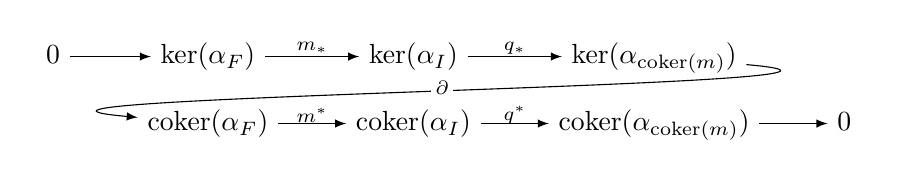
\begin{tikzpicture}[descr/.style={fill=white,inner sep=1.5pt}]
    \matrix (m) [ matrix of math nodes, row sep=1em, column sep=2.5em, text height=1.5ex, text
    depth=0.25ex ]
    { 0 & \ker(\alpha_F) & \ker(\alpha_I) & \ker(\alpha_{\coker(m)}) & \\
      & \coker(\alpha_F) & \coker(\alpha_I) & \coker(\alpha_{\coker(m)}) & 0 \\
    };

    \path[overlay,->, font=\scriptsize,>=latex] (m-1-1) edge (m-1-2) (m-1-2) edge
    node[yshift=0.7ex]{$m_{\ast}$} (m-1-3) (m-1-3) edge
    node[yshift=0.7ex]{$q_{\ast}$} (m-1-4) (m-1-4) edge[out=355,in=175] node[descr,yshift=0.3ex]
    {$\partial$} (m-2-2) (m-2-2) edge
    node[yshift=0.7ex]{$m^{\ast}$} (m-2-3) (m-2-3) edge
    node[yshift=0.7ex]{$q^{\ast}$} (m-2-4) (m-2-4) edge (m-2-5);
  \end{tikzpicture}
\]
But we see from the definition of $\lim$ that the kernels of $\alpha$ are precisely the $\lim$. Thus
we have the following long exact sequence.
\[
  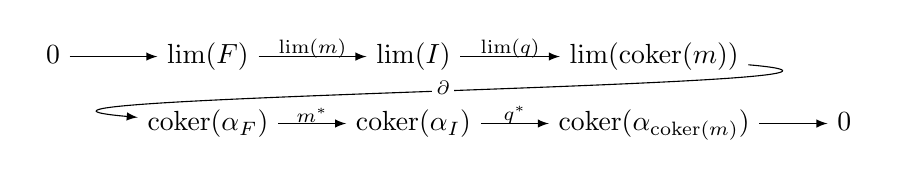
\begin{tikzpicture}[descr/.style={fill=white,inner sep=1.5pt}]
    \matrix (m) [ matrix of math nodes, row sep=1em, column sep=2.5em, text height=1.5ex, text
    depth=0.25ex ]
    { 0 & \lim(F) & \lim(I) & \lim(\coker(m)) & \\
      & \coker(\alpha_F) & \coker(\alpha_I) & \coker(\alpha_{\coker(m)}) & 0 \\
    };

    \path[overlay,->, font=\scriptsize,>=latex] (m-1-1) edge (m-1-2) (m-1-2) edge
    node[yshift=0.7ex]{$\lim(m)$} (m-1-3) (m-1-3) edge
    node[yshift=0.7ex]{$\lim(q)$} (m-1-4) (m-1-4) edge[out=355,in=175] node[descr,yshift=0.3ex]
    {$\partial$} (m-2-2) (m-2-2) edge
    node[yshift=0.7ex]{$m^{\ast}$} (m-2-3) (m-2-3) edge
    node[yshift=0.7ex]{$q^{\ast}$} (m-2-4) (m-2-4) edge (m-2-5);
  \end{tikzpicture}
\]

The last step in the proof will be to show that $\coker(\alpha_I)$ is $0$, in which case
${\lim}^1(F)$ is isomorphic to $\coker(\alpha_F)$. Showing that $\coker(\alpha_I)$ is $0$ is
equivalent to showing that $\alpha_I$ is surjective. To see this, pick any element
$(j_0, j_1, j_2, \ldots) \in \prod_i I_i$. We need to find an element $(k_0, k_1, k_2, k_3, \ldots)$
such that we have the following equalities.
\begin{align*}
  j_0 &= k_0 - i_1(k_1) \\
  j_1 &= k_1 - i_2(k_2) \\
  j_2 &= k_2 - i_3(k_3) \\
      &\vdots
\end{align*}
But notice that we constructed $I$ such that all the $i_k$ are surjective. That means this system of
equations can be solved simultaneously and $\coker(\alpha_I)$ is $0$. This shows the result.

\end{proof}

\begin{thm}[Milnor exact sequence] \label{thm-milnor} If $\{ i_n : X_n \hookrightarrow X_{n+1} \}$
  for $n \in \mathbb{N}$ are a sequence of nested (pointed) CW subcomplexes such that
  $X = \bigcup_n X_n$, and $\redco^{\ast}$ is a reduced cohomology theory, then we have the
  following exact sequence for all $i \geq 1$.
  \begin{align*}
    0 \rightarrow {\lim_{n}}^1 \redco^{i-1}(X_n) \rightarrow \redco^i(X) \rightarrow \lim_n \redco^i(X_n) \rightarrow 0
  \end{align*}
\end{thm}

\begin{proof}
  We first construct the mapping telescope of the inclusions. We start with the (unpointed) space
  $X \times \mathbb{R}_+$.  We then consider the following subspace $S$.
  \begin{align*}
    S = \bigcup_{i \in \mathbb{N}} X_i \times [i,i+1]
  \end{align*}
  We then quotient $S$ by the subspace ${\ast} \times \mathbb{R}_+$ and we use the quotient out
  space as the basepoint of the pointed mapping telescope $T$.

  We define two subspaces of the mapping telescope; we'll apply Mayer-Vietoris to these subspaces.
  \begin{align*}
    T_1 &:= \bigcup_{i \in \mathbb{N}} X_{2i+1} \times [2i+1, 2i+2] \\
    T_2 &:= \bigcup_{i \in \mathbb{N}} X_{2i} \times [2i, 2i+1] 
  \end{align*}
  To be more precise, we should be taking open neighbourhoods of these spaces to apply
  Mayer-Vietoris, but the open neighbourhoods deformation retract to these spaces anyways, so it's
  alright.  Observe that the intersection $T_0$ of $T_1$ and $T_2$ is homeomorphic to the wedge of
  all the $X_i$.  By similar reasoning (although we replace homeomorphism by homotopy equivalence),
  we get that $T_1$ is homotopy equivalent to the wedge of all the $X_i$ for odd $i$ and $T_2$ the
  wedge of $X_i$ for all even $i$. We consider the Mayer-Vietoris sequence, and use the
  $(\mathrm{DV})$ axiom to get isomorphisms.
  \[
    \begin{tikzcd}
      \redco^{q+1}(T) & \redco^{q}(T_0) \ar[l] \ar[d, "\cong"] & \redco^{q}(T_1) \oplus \redco^{q}(T_2) \ar[l, swap, "\phi_q"] \ar[d, "\cong"] & \redco^{q+1}(T) \ar[l] \\
      & \prod_{i \in \mathbb{N}} \redco^{q}(X_i) \ar[dl, swap, "\cdot (-1)^i"] & \prod_{i \in \mathbb{N}} \redco^{q}(X_{2i}) \oplus \prod_{i \in \mathbb{N}} \redco^{q}(X_{2i+1}) \ar[dll, "m_q"] &   \\
      \prod_{i \in \mathbb{N}} \redco^{q}(X_i) & & & \\
    \end{tikzcd}
  \]
  We need to determine how the map $m_q$ should be defined to make the diagram commute.  We do this
  by seeing how the map behaves on the basis. First, we take $x_0 \in \redco^{q}(X_0)$. The first
  isomorphism takes it to $(x, 0)$, the map $\phi_q$ takes it $x-0$ and finally it goes to
  $x$. Next, we see how $x_1 \in \redco^{q}(X_1)$ behaves. It first gets sent to
  $(i_0^{\ast}x_1, x_1)$ and then to $i_0^{\ast}x_1 - x_1$.  Finally, the $(-1)^i$ sends it to
  $x_1 - i_0^{\ast}x_1$. Similarly, $x_2 \in \redco^{q}(X_2)$ gets sent to $x_2-i_1^{\ast}x_2$, and
  so go on the rest of the basis elements. We now have the following long exact sequence.
  \[
    \begin{tikzcd}
      \redco^{q+1}(T) & \prod_{i \in \mathbb{N}}\redco^{q} (X_i) \ar[l] & \prod_{i \in \mathbb{N}}\redco^{q} (X_i) \ar[swap, l, "m_q"] & \redco^{q}(T) \ar[l] \\
    \end{tikzcd}
  \]

  From this, we get the following short exact sequence.
  \[
    \begin{tikzcd}
      0 & \ker(m_q) \ar[l] & \redco^{q}(T) \ar[l] & \coker(m_{q-1}) \ar[l] & 0 \ar[l] \\
    \end{tikzcd}
  \]
  From theorem \ref{thm-lim1}, we see that $\ker(m_q)$ is $\lim_n(\redco^{q}(X_n))$ and
  $\coker(m_{q-1})$ is ${\lim_n}^1(\redco^{q-1}(X_n))$. This proves the theorem.

\end{proof}

\bibliography{references}
\bibliographystyle{amsplain}

\end{document}
